\documentclass[a4paper,12pt,usenames,dvipsnames]{beamer}
\usepackage[utf8]{inputenc}
\usepackage[T1]{fontenc}
\usepackage[french]{babel}
\usepackage{xcolor}
\usepackage{pifont}
\usetheme{Singapore} %Boadilla | Bergen | Madrid | Antibes | Hannover | Singapore | Warsaw

\newcommand{\cmark}{\ding{51}}
\newcommand{\xmark}{\ding{55}}
%----------------------------------------------------------------------------------------
%   TITLE INFORMATION
%----------------------------------------------------------------------------------------
\title{Entrepôts de données pour \textit{Tam voyages}}
\subtitle{HMIN122M -- Entrepôts de Données et Big-Data}
\author{B. Rima \and J. Saba \and T. Shaqura \and J. Bourgin}
\institute[UM]{M1 Informatique AIGLE}
\date{\today}
\logo{
\includegraphics[scale=0.2]{images/umLogo.png}}

%----------------------------------------------------------------------------------------
%   OUTLINE
%----------------------------------------------------------------------------------------
\AtBeginSection[]{
  \begin{frame}{Sommaire}
  \tableofcontents[currentsection]
  \end{frame}
}

\begin{document}
%----------------------------------------------------------------------------------------
%   TITLE FRAME
%----------------------------------------------------------------------------------------
\begin{frame}
\titlepage
\end{frame}
%----------------------------------------------------------------------------------------
%   INTRODUCTION
%----------------------------------------------------------------------------------------
\section{Introduction}
\begin{frame}{Objectifs de \textit{tam-voyages}}{Introduction}
\begin{itemize}
  \item<1-> augmenter le taux de vente des tickets;
  \item<2-> augmenter le taux d'abonnements;
  \item<3-> améliorer la qualité de service;
  \item<4-> réduire les dépenses;
  \item<5-> $\dots$
\end{itemize}
\end{frame}

\begin{frame}{Problématiques}{Introduction}
  \begin{block}{Problématique 1}
    \og \textit{Comment peut-on tirer partie de la fréquentation des véhicules en se basant sur la circulation du réseau afin d'améliorer la qualité de service ?} \fg
  \end{block}

  \begin{block}{Problématique 2}
    \og \textit{Comment peut-on suivre l'évolution et la maintenance des matériaux de manière à réduire les dépenses associées ?} \fg
  \end{block}
\end{frame}

\begin{frame}{Actions et opérations possibles par \textit{tam-voyages}}{Introduction}
  \begin{itemize}
    \item<1-> \textcolor{OliveGreen}{voyages};
    \item<2-> \textcolor{OliveGreen}{maintenance de véhicules};
    \item<3-> vente de tickets et abonnements;
    \item<4-> amendes;
    \item<5-> $\dots$
  \end{itemize}
\end{frame}

\begin{frame}{Actions et opérations considérées}{Introduction}
  \begin{block}{Voyages}
    \texttt{Le voyage d'un voyageur via un véhicule d'une ligne du réseau à une heure et une date donnée}.
  \end{block}

  \begin{examples}
    \begin{itemize}
      \item<1-> \textit{le nombre de voyages utilisant des tickets par chaque bus pour le mois de juillet}
      \item<2-> \textit{l'arrêt le plus fréquenté par chaque ligne du réseau}
    \end{itemize}
  \end{examples}
\end{frame}

\begin{frame}{Actions et opérations considérées}{Introduction}
  \begin{block}{Maintenance de véhicules}
    \texttt{Chaque transaction effectuée lors de la maintenance d'un véhicule à une heure et une date donnée}.
  \end{block}

  \begin{examples}
    \begin{itemize}
      \item<1-> \textit{le coût total de maintenance de chaque véhicule}
      \item<2-> \textit{le nombre total de maintenances effectuées par véhicule pour les 6 dernier mois.}
    \end{itemize}
  \end{examples}
\end{frame}

\section{Modélisation}
\begin{frame}{Contexte du projet}{Introduction}
\end{frame}

\section{Implémentation}
\begin{frame}{Implémentation}{Technologie choisie}
\begin{figure}[!ht]
  \centering
  
\includegraphics[scale=0.2]{images/Oracle.png}
  \caption{What else besides Oracle?}
\end{figure}
\end{frame}

\begin{frame}{Implémentation}{Quelques résultats (\texttt{Voyage})}
  \begin{figure}[!ht]
    \centering
    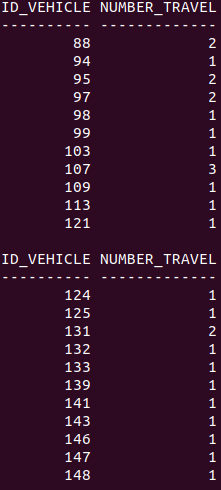
\includegraphics[scale=0.3]{images/requetes_analytiques/requ1.png}
    \caption{le nombre de voyages utilisant des tickets par chaque bus pour le mois de juillet}
  \end{figure}
\end{frame}

\begin{frame}{Implémentation}{Quelques résultats (\texttt{Voyage})}
\begin{figure}[!ht]
  \centering
  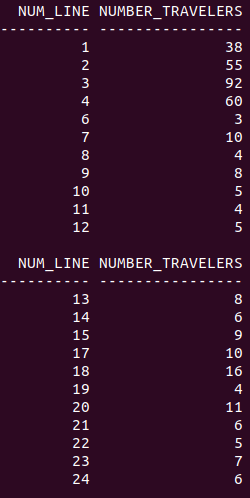
\includegraphics[scale=0.3]{images/requetes_analytiques/requ2.png}
  \caption{le nombre de voyageurs abonnés par ligne pour chaque voyage pour les deux derniers mois}
\end{figure}
\end{frame}

\begin{frame}{Implémentation}{Quelques résultats (\texttt{Voyages})}
\begin{figure}[!ht]
  \centering
  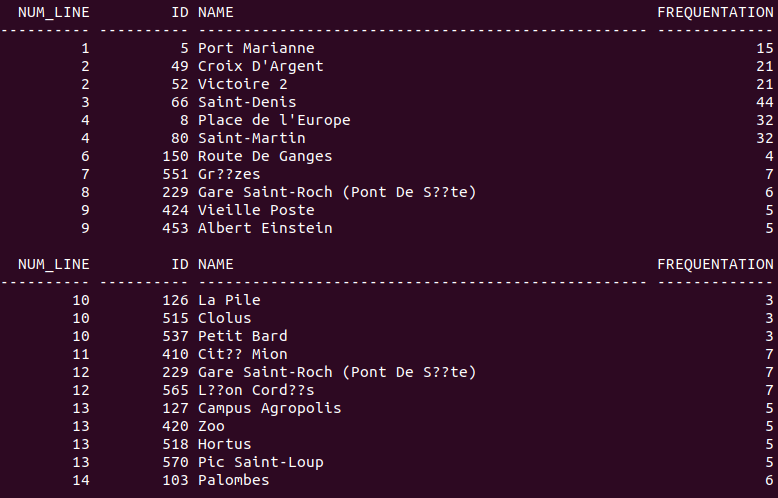
\includegraphics[scale=0.3]{images/requetes_analytiques/requ3.png}
  \caption{l'arrêt le plus fréquenté par ligne}
\end{figure}
\end{frame}

\begin{frame}{Implémentation}{Quelques résultats (\texttt{Maintenance})}
\begin{figure}[!ht]
  \centering
  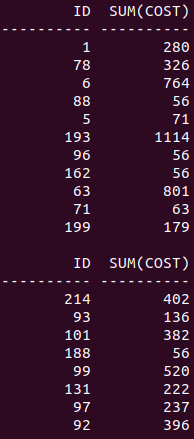
\includegraphics[scale=0.3]{images/requetes_analytiques/requ6.png}
  \caption{le coût total de maintenance de chaque véhicule}
\end{figure}
\end{frame}

\begin{frame}{Implémentation}{Quelques résultats (\texttt{Maintenance})}
\begin{figure}[!ht]
  \centering
  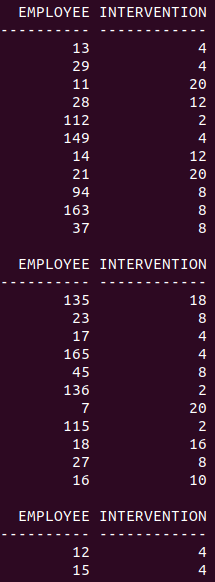
\includegraphics[scale=0.25]{images/requetes_analytiques/requ7.png}
  \caption{le nombre de maintenances effectuées sur les bus par employé pour l'année 2018}
\end{figure}
\end{frame}

\section{Conclusion}
\begin{frame}{Conclusion}{Perspectives}
  Bien que notre entrepôt permet de réaliser des analyses primordiales, nous avons constaté qu’il était assez limité tel que :
  \begin{itemize}
    \item il est incapable d'approximer le chiffre d’affaires de \textit{tam-voyages} en termes de ventes de tickets et d'abonnements.
    \item il ne permet pas de connaître et d'analyser les détails de fréquentation de chaque trajet effectué par un véhicule.
  \end{itemize}
\end{frame}

\begin{frame}{Conclusion}{\textit{Data mart} pour la vente des tickets}
  \begin{block}{Fait}
    La vente d'un ticket via une borne de vente à une date donnée, avec une mesure désignant le prix du ticket vendu
  \end{block}

  \begin{block}{Dimensions}
    \begin{itemize}
      \item voyageur
      \item date
      \item borne de vente
    \end{itemize}
  \end{block}
\end{frame}

\begin{frame}{Conclusion}{\textit{Data mart} pour les abonnements}
  \begin{block}{Fait}
    L'abonnement d'un voyageur à une date donnée, avec des mesures désignant les frais de l'abonnement et sa durée de validité
  \end{block}

  \begin{block}{Dimensions}
    \begin{itemize}
      \item voyageur
      \item date
    \end{itemize}
  \end{block}
\end{frame}

\begin{frame}{Conclusion}{\textit{Data mart} pour les trajets effectués par des véhicules}
  \begin{block}{Fait}
    Un trajet effectué par un véhicule sur une ligne du réseau de transport à une heure et une date données, sans aucune mesure explicite.
  \end{block}

  \begin{block}{Dimensions}
    Les mêmes dimensions de la table \texttt{Voyage}, avec liaison de la table \texttt{Trajet} à cette dernière pour raffiner les analyses de manière à inclure des informations supplémentaires sur les trajets.
  \end{block}
\end{frame}
\end{document}
